\documentclass[a4paper,12pt,dvipsnames]{article}%
\usepackage{amsmath}%
\usepackage{amsfonts}%
\usepackage{amssymb}%
\usepackage{mathtools}
\usepackage{graphicx}
\usepackage{geometry}
\usepackage[hidelinks]{hyperref}
\usepackage{svg}
\usepackage{longtable}
\usepackage{array}
\usepackage{float}
\usepackage{pdflscape}
\usepackage{listings}
\usepackage[T1]{fontenc}
\usepackage{textcomp}
\usepackage[parfill]{parskip}
\usepackage[toc,page]{appendix}
\usepackage{url}
\usepackage{enumitem}
\geometry{margin=1in}
\makeatletter\let\MPtrue\@minipagetrue\makeatother
\usepackage{ragged2e}
\usepackage{xkeyval}
\usepackage{nicefrac}
\usepackage{lmodern}
\usepackage{lscape}
\usepackage{microtype}

\DeclarePairedDelimiter{\ceil}{\lceil}{\rceil}

\newcolumntype{x}[1]{>{\raggedright\centering\arraybackslash\hspace{0pt}}p{#1}}
\newcolumntype{M}[1]{>{\raggedright\centering\arraybackslash\hspace{0pt}}m{#1}}
\newcolumntype{R}[1]{>{\RaggedLeft\arraybackslash}p{#1}}

\makeatletter

\define@cmdkey      [CDK] {ccd}     {name}      {}
\define@cmdkey      [CDK] {ccd}     {vldesc}    {}
\define@cmdkey      [CDK] {ccd}     {ldesc}     {}
\define@cmdkey      [CDK] {ccd}     {ndesc}     {}
\define@cmdkey      [CDK] {ccd}     {hdesc}     {}
\define@cmdkey      [CDK] {ccd}     {vhdesc}    {}
\define@cmdkey      [CDK] {ccd}     {ehdesc}    {}

\define@cmdkey      [CDK] {ccd}     {vlmult}    {}
\define@cmdkey      [CDK] {ccd}     {lmult}     {}
\define@cmdkey      [CDK] {ccd}     {nmult}     {}
\define@cmdkey      [CDK] {ccd}     {hmult}     {}
\define@cmdkey      [CDK] {ccd}     {vhmult}    {}
\define@cmdkey      [CDK] {ccd}     {ehmult}    {}

\newcommand{\cdtable}[1]{%
	\setkeys[CDK]{ccd}{#1}
\begin{table}[H]
	\centering
	\begin{tabular}{|M{0.165\linewidth}|M{0.125\linewidth}|M{0.125\linewidth}|M{0.125\linewidth}|M{0.125\linewidth}|M{0.125\linewidth}|M{0.125\linewidth}|}
		\hline
		\textbf{\cmdCDK@ccd@name \break Descriptors:} & {\small \cmdCDK@ccd@vldesc} & {\small \cmdCDK@ccd@ldesc} & {\small \cmdCDK@ccd@ndesc} & {\small \cmdCDK@ccd@hdesc} & {\small \cmdCDK@ccd@vhdesc} & {\small \cmdCDK@ccd@ehdesc} \\
		\hline
		\textbf{Rating Level} & Very Low & Low & Nominal & High & Very High & Extra High \\
		\hline
		\textbf{Effort Multipliers} & \cmdCDK@ccd@vlmult & \cmdCDK@ccd@lmult & \cmdCDK@ccd@nmult & \cmdCDK@ccd@hmult & \cmdCDK@ccd@vhmult & \cmdCDK@ccd@ehmult \\
		\hline
	\end{tabular}
	\caption{\cmdCDK@ccd@name \ Cost Driver}
\end{table}
}

\makeatother

\sloppy
\begin{document}
	\begin{figure}
  \centering
	\def\svgwidth{\columnwidth}
    \resizebox{0.35\textwidth}{!}{\input{logo_polimi.pdf_tex}}
\end{figure}
\title{{\Huge \textbf{D}esign \textbf{D}ocument}\\{\Large Software Engineering 2: ``myTaxiService''}}

\author{Fioratto Raffaele, Longoni Nicol\`{o}
\\Politecnico di Milano
\\{\small A.Y. 2015/2016}}
\date{November 14, 2015}
\maketitle
\newpage
\tableofcontents
	\section{Introduction}
\subsection{Purpose}
This documentation represents the Design Document (DD). It describes completely the system in terms of components, analyzing their internal and external interactions (with the actors). It starts off with the description of the system given in the Requirements Analysis and Specification Document. In this document the system is treated like a white box, i.e. the document ``opens" it and then dissects it starting with a high level overview to a more detailed representation. This document is addressed to all developers and programmers who have to implement the actual software.
\subsection{Scope}
The aim of the project is to create a new brand system that optimizes an 
existing taxi service.
The system will be capable of automatizing and/or simplifying certain 
processes during requests or reservations of taxis.
It will also guarantee a fair management of taxi queues.
New passengers can sign up for service inserting some basic information in order to use service's features as soon as possible.
A passenger can request a taxi using web service or through mobile
application after registration. The system will be able to localize precisely the position
of the passenger, determining taxis that are available near
him/her. The system will select a taxi and then it will forward the request to one of its driver.
Upon confirmation, the system will notify the customer about the successful completion of the operation and the ETA of the taxi. A passenger can also reserve a taxi by specifying time and date, but they have to do it with at least two hours in advance. Cancellation is also permitted. The system will actually process the request ten minutes before the time specified during the reservation in the same way as described previously.
\subsection{Definitions, Acronyms, Abbreviations}
\subsubsection{Definitions}
\subsubsection{Acronyms}
\begin{itemize}
	\item DD: Design Document
	\item RASD: Requirement Analysis and Specification Document
	\item MVC: Model View Controller
	\item SOA: Service Oriented Application
	\item JEE: Java Enterprise Edition
	\item FSA: Finite State Automaton
\end{itemize}
\subsubsection{Abbreviations}
\subsection{Reference Documents}
\begin{itemize}
	\item myTaxiService Specification Document
	\item myTaxiService RASD
	\item DD Structure Template
\end{itemize}
\subsection{Document Structure}
\begin{itemize}
	\item Section 1: Introduction, it gives a description of this document, some basic information in order to clearly understand the subsequent sections.
	\item Section 2: Architectural Design, it describes the software to be designed starting with a high level representation and then dissecting it providing a more detailed analysis. Diagrams are provided to better clarify this part.
	\item Section 3: Algorithm Design: it gives a description of the main algorithms that are implemented in the software, pseudo-code or flow diagrams are provided to describe them in a more clear way.
	\item Section 4: User Interface Design: starting with mockups presented in the RASD, this part further explains interactions between actors and the system, and shows how it will look like.
	\item Section 5: Requirements Traceability: this part explains how requirements defined in the RASD map into the design elements that we shall define in this document.
	\item Section 6: References: this section provides a list of external documents and materials that allowed the composition of this documentation.
\end{itemize}
	\newpage
\def\arraystretch{1.15}
\section{Cost Estimation}
\subsection{Function Points}
\subsubsection{Brief introduction}
The Function Point estimation approach, is based on the principle of extracting functions from a software, classify them using a well defined set classes and estimate their complexity. \\ This kind of estimation is extremely useful since it can be done at a very early stage of a project life-cycle, ideally after the implementation of the RASD, moreover, it can be used as a basis for performing a cost estimation using well-known models such as COCOMO (explained later on). \\
This estimation is a single number called UFP that can be computed using simple arithmetic. \\
An high-level procedure of how to calculate this number is the following:
\begin{enumerate}
	\item Classify each function of the software to one of this possible five classes called Function Types (explained in detail later):
	\begin{itemize}
		\item Internal Logic Files
		\item External Interfaces Files
		\item External Inputs
		\item External Outputs
		\item External Inquiries
	\end{itemize}
	\item For each function define its complexity which can be:
	\begin{itemize}
		\item Low
		\item Average
		\item High
	\end{itemize}
	\item Calculate the UFC by using this formula:
	$$ \sum_{f \in F,\ c \in C} \left((\textrm{\# of functions of type } f \textrm{ and complexity } c) \cdot (\textrm{weight for type } f \textrm{ and complexity } c ) \right) $$
	where $F = $ \{ILF, ELF, EI, EO, EIQ\} and $C = $ \{Low, Average, High\}. \\
	Refer to this table for determine the proper weight for each type and complexity:
	\begin{table}[H]
	\centering
	\begin{tabular}{x{0.3\linewidth}x{0.15\linewidth}x{0.15\linewidth}x{0.15\linewidth}}
		\hline 
		& \multicolumn{3}{c}{\textbf{Complexity-Weight}} \\
		\textbf{Function Type} & \textbf{Low} &\textbf{Average} & \textbf{High} \\
		\hline
		Internal Logical Files & 7 & 10 & 15 \\
		External Interfaces Files & 5 & 7 & 10 \\
		External Inputs & 3 & 4 & 6 \\
		External Outputs & 4 & 5 & 7 \\
		External Inquiries & 3 & 4 & 6 \\
		\hline
	\end{tabular}
	\caption{UFP Complexity Weights}
\end{table}
\end{enumerate}
Further manipulation of the UFP can be done in order to use it in Cost Estimation Models such as COCOMO, but this will be explained later.
\subsubsection{Internal Logic Files}
The application should manage an internal database which it is used to store information about the three categories of registered users: Passengers, Taxi Drivers, Sys Admins. For each of them basic data it is collected: name, surname, password, e-mail and so on. Thus we think that the complexity for this entities should be set to \textbf{Low}. On the other hand the system also maintain a history of Rides carried out throughout its life-cycle, since this entity is a bit complex than the previous ones we set its complexity to \textbf{Average}.
\begin{table}[H]
	\centering
	\begin{tabular}{p{0.5\linewidth}x{0.2\linewidth}R{0.3\linewidth}}
		\hline
		\textbf{ILF} & \textbf{Complexity} & \textbf{FP} \\ \hline
		Passengers & Low & 7 \\
		Taxi Drivers & Low & 7 \\
		Sys Admins & Low & 7 \\
		Rides & Average & 10 \\
		\multicolumn{2}{l}{\textbf{Total}} & 31 \\
		\hline
	\end{tabular}
	\caption{ILFs Table Recap}
\end{table}
\subsubsection{External Logic Files}
The application should interact with a Maps service which provides information regarding city map and ETAs of Rides. This interaction requires the understanding of some API(s) and the need of parsing data coming from the Internet so we set this function complexity to \textbf{Average}. \\ Another interaction is with an external Database containing various information about Cars and Drivers, this interaction is simpler than the previous one and, by the way, Java has already well-defined interfaces to dialog with a Database so we set the complexity to \textbf{Low}.  
\begin{table}[H]
	\centering
	\begin{tabular}{p{0.5\linewidth}x{0.2\linewidth}R{0.3\linewidth}}
		\hline
		\textbf{ELF} & \textbf{Complexity} & \textbf{FP} \\ \hline
		Maps Service & Average & 7 \\
		Cars and Drivers Database & Low  & 5 \\
		\multicolumn{2}{l}{\textbf{Total}} & 12 \\
		\hline
	\end{tabular}
	\caption{ELFs Table Recap}
\end{table}
\subsubsection{External Inputs}
The application has to deal with this external interactions from the users:
\begin{itemize}
	\item \textit{Login/logout}, these are a simple operations (they are two distinct functions) so we can set their complexity to \textbf{Low}.
	\item \textit{Passenger/Taxi Driver registration}, as for the previous functions, these are simple too, so their complexity is again \textbf{Low}.
	\item \textit{Perform Request/Reservation}, these are the most complex operations since several components are involved and some of them are also external, so we set their complexity to \textbf{High}.
	\item \textit{Accept Request from Taxi Driver/Passenger}, these operations involve a medium number of components, also interacts with the internal database in order to add relevant information to Rides history, thus the complexity is set to \textbf{Average}.
	\item \textit{Modify Passenger's profile}, this is a simple operation, complexity is \textbf{Low}.
	\item \textit{Change Taxi Driver's status}, this requires to remove/add the Taxi to the proper queue, but nevertheless this is a fairly simple operations, so the complexity is \textbf{Low}.
\end{itemize} 
\begin{table}[H]
	\centering
	\begin{tabular}{p{0.5\linewidth}x{0.2\linewidth}R{0.3\linewidth}}
		\hline
		\textbf{EI} & \textbf{Complexity} & \textbf{FP} \\ \hline
		Login & Low & 3 \\
		Logout & Low & 3 \\
		Passenger Registration & Low & 3 \\
		Taxi Driver Registration & Low & 3 \\
		Perform Request & High & 6 \\
		Perform Reservation & High & 6 \\ 
		Accept Request from Taxi Driver & Average & 4 \\ 
		Accept Request from Passenger & Average & 4 \\
		Modify Passenger's Profile & Low & 3 \\ 
		Change Taxi Driver's status & Low & 3 \\
		\multicolumn{2}{l}{\textbf{Total}:} & 38 \\
		\hline
	\end{tabular}
	\caption{EIs Table Recap}
\end{table}
\subsubsection{External Outputs}
The applications generates the following complex outputs to the users:
\begin{itemize}
	\item \textit{Propose Ride to Taxi Driver/Passenger}, this is a fairly simple operation once the overall elaboration and computation has been done on the back-end, so we set the complexity to \textbf{Low}.
	\item \textit{Calculate ETA}, for this function a bunch of input data has to be collected from the environment (GPS positions), and an external service must be contacted, which computes the actual result, so we set the complexity of this to \textbf{Average}.
	\item \textit{Select Best Taxi for Incoming Ride}, this depends to the policies chosen for managing queues in terms of assignment to city map and algorithm for taxi selection from a specific queue. We set the complexity of this function to \textbf{Average}. 
\end{itemize}
\begin{table}[H]
	\centering
	\begin{tabular}{p{0.5\linewidth}x{0.2\linewidth}R{0.3\linewidth}}
		\hline
		\textbf{EO} & \textbf{Complexity} & \textbf{FP} \\ \hline
		Propose Ride to Taxi Driver & Low & 4 \\
		Propose Ride to Passenger & Low & 4 \\
		Calculate ETA & Average & 5 \\
		Select Best Taxi for Incoming Ride & Average & 5 \\		
		\multicolumn{2}{l}{\textbf{Total}} & 18 \\
		\hline
	\end{tabular}
	\caption{EOs Table Recap}
\end{table}
\subsubsection{External Inquiries}
The application allows users to requests informations about themselves and other things but all of them are simple to implement, so their complexity is set to \textbf{Low}. 
\begin{table}[H]
	\centering
	\begin{tabular}{p{0.5\linewidth}x{0.2\linewidth}R{0.3\linewidth}}
		\hline
		\textbf{EIQ} & \textbf{Complexity} & \textbf{FP} \\ \hline
		Show Passenger's Profile & Low & 3 \\
		Show Taxi Driver's Profile & Low & 3 \\
		Show Sys Admin's Profile & Low & 3 \\
		Show ETA & Low & 3 \\
		\multicolumn{2}{l}{\textbf{Total}} & 12 \\
		\hline
	\end{tabular}
	\caption{EIQs Table Recap}
\end{table}
\subsubsection{Recap}
The following table summarize the amount of FP for each type and the overall sum that corresponds to the final UFP value.
\begin{table}[H]
	\centering
	\begin{tabular}{p{0.7\linewidth}R{0.3\linewidth}}
		\hline
		\textbf{Function Type} & \textbf{Value} \\ \hline
		Internal Logic Files & 31 \\
		External Logic Files & 12 \\
		External Inputs & 38 \\
		External Outputs & 18 \\
		External Inquiries & 12 \\
		\textbf{Total (UFP)} & 111 \\
		\hline
	\end{tabular}
	\caption{Final FPs recap with UFP calculation}
\end{table}
\subsection{COCOMO}
\subsubsection{Brief introduction}
\label{sec:cocomo-int}
This estimation is achieved using a complex, non linear model that takes into account the characteristic of the product but also of people and process. \\
Basically, this model estimates the effort needed to implement the project being analyzed. To compute this number we need to define some concept which will be used later in the actual calculation. \\
The equation to compute the effort is the following:
$$\textrm{Effort} = A \cdot \textrm{SLOC}^E \cdot \prod_{i=1}^{n} EM_i$$
Where $A = 2.94$ for COCOMO II.2000, SLOC is the amount of lines of codes estimated to be written for implementing the software, $E$ is explained in detail in Section \ref{sec:sd} and $EM$ is called effort multiplier which is defined for each Cost Driver (explained in Section \ref{sec:cd}), in COCOMO II.2000 the number of Cost Driver are 17 thus $n = 17$.
\subsubsection{Lines of Codes}
This datum can be determined using a simple conversion equation of this kind
$$ \textrm{SLOC} = k \cdot \textrm{UFP} $$
Where $k$ is a coefficient which is assigned given the programming language chosen for implementing the software, in our case the language is Java thus $k = 53\ \nicefrac{\textrm{SLOC}}{\textrm{UFP}}$. \\
Given this information, we can estimate our SLOC for the sotware which is:
$$SLOC = 53 \cdot 111 = 5,883 = 5.88\ KSLOC$$
This value will be used later for computing the effort.
\subsubsection{Scale Drivers}
The exponent $E$ in the equation of the Effort is an aggregation of five \textit{scale factors} (SF) that account
for the relative economies or diseconomies of scale encountered for software projects of different
sizes. \\
If $E < 1.0$, the project exhibits economies of scale. If the product's
size is doubled, the project effort is less than doubled. The project's productivity increases as the
product size is increased. \\
If $E = 1.0$, the economies and diseconomies of scale are in balance. This linear model is
often used for cost estimation of small projects. \\
If $E > 1.0$, the project exhibits diseconomies of scale. This is generally because of two
main factors: growth of interpersonal communications overhead and growth of large-system
integration overhead. \\
$E$ can be computed using this equation:
$$ E = B + 0.01 \cdot \sum_{j=1}^{5} \textrm{SF}_j $$
where $B = 0.91$ (for COCOMO II.2000). \\
Scale Factors are defined in the following table:
\label{sec:sd}
\begin{table}[H]
	\centering
	\begin{tabular}{|x{0.11\linewidth}|x{0.135\linewidth}|x{0.125\linewidth}|x{0.13\linewidth}|x{0.13\linewidth}|x{0.13\linewidth}|x{0.135\linewidth}|}
		\hline
		\textbf{Scale Factors} & \textbf{Very Low} & \textbf{Low} & \textbf{Nominal} & \textbf{High} & \textbf{Very High} & \textbf{Extra High} \\ \hline
		\textbf{\uppercase{Prec}:} & Thoroughly unprecedented & Largely unprecedented & Somewhat unprecedented & Generally familiar & Largely familiar & Thoroughly familiar \\
		\textbf{SF\textsubscript{i}:} & 6.20 & 4.96 & 3.72 & 2.48 & 1.24 & 0.00 \\
		\hline
		\textbf{FLEX:} & Rigorous & Occasional relaxation & Some relaxation & General conformity & Some conformity & General goals \\
		\textbf{SF\textsubscript{i}:} & 5.07 & 4.05 & 3.04 & 2.03 & 1.01 & 0.00 \\
		\hline
		\textbf{RESL:} & Little (20\%) & Some (40\%) & Often (60\%) & Generally (75\%) & Mostly (90\%) & Full (100\%) \\
		\textbf{\textbf{SF\textsubscript{i}:}} & 7.07 & 5.65 & 4.24 & 2.83 & 1.41 & 0.00 \\
		\hline 
		\textbf{TEAM:} & Very difficult interactions & Some difficult interactions & Basically cooperative interactions & Largely cooperative & Highly cooperative & Seamless interactions \\
		\textbf{\textbf{SF\textsubscript{i}:}} & 5.48 & 4.38 & 3.29 & 2.19 & 1.10 & 0.00 \\
		\hline
		& \multicolumn{6}{c|}{The estimated Equivalent Process Maturity Level (EPML) or} \\
		\cline{2-7}
		\textbf{PMAT:} & SW-CMM Level 1 Lower & SW-CMM Level 1 Upper & SW-CMM Level 2 & SW-CMM Level 3 & SW-CMM Level 4 & SW-CMM Level 5 \\
		\textbf{\textbf{SF\textsubscript{i}:}} & 7.80 & 6.24 & 4.68 & 3.12 & 1.56 & 0.00 \\
		\hline
	\end{tabular}
	\caption{Scale Factor Values, SF\textsubscript{i}, for COCOMO II Models}
\end{table}
According to the table we can evaluate the scale factors for our project:
\begin{itemize}
	\item \textbf{Precedentedness}, it measures the previous experience that we had with this kind of technologies. Since this is our first project using JEE and these development methodologies, we set it to \textbf{Low}. 
	\item \textbf{Development flexibility}, its value express the degree of elasticity that we have during the development of the project, in particular it depends on how the software needs to be conformant to pre-established requirements, with external interface specifications and so on. Since the original project specification explains the problems without going too much in detail, this induces us to set this value to Extra High, however during the implementation of the RASD, some requirements expressed the need to interact with some external component which have a fixed and already established interface. Thus, we decide to adjust this SF to a more fair value of \textbf{High}.
	\item \textbf{Risk resolution}, it reflects the amount of effort and budget expected to be spent during the development to seek for possible risks and their resolution that can occur anytime during the life-cycle of a software. All the documents written till now don't carry out this type of problems, the PPD has a dedicated section explain to some extent this kind of issues, so we can set this SF to \textbf{Nominal}.
	\item \textbf{Team cohesion}, it measures the overall capabilities of all actors (users, customers, developers, maintainers, etc.) of the development process to interact each other to carry out the main objectives. Since in our case, the team is composed of only two members, that already worked together to other projects in the past, we set this value to \textbf{Very High}.
	\item \textbf{Process maturity}, it is an indicator of how the overall process of development is sophisticated and well-defined with the respect to some general criteria. Since precise instructions has been given for each phase of the project we set it to \textbf{High} (CMM Level 3). 
\end{itemize}

The results are recapped in the following table:
\begin{table}[H]
	\centering
	\begin{tabular}{p{0.5\linewidth}x{0.2\linewidth}R{0.3\linewidth}}
		\hline
		\textbf{Scale Driver} & \textbf{Selected Factor} & \textbf{Value} \\
		\hline
		Precedentness & Low & 4.96 \\
		Development Flexibility & High & 2.03 \\
		Risk Resolution & Nominal & 4.24 \\
		Team Cohesion & Very High & 2.19 \\
		Process Maturity & High & 3.12 \\
		\multicolumn{2}{l}{\textbf{Total}} & 16.60 \\
		\hline
	\end{tabular}
\end{table}

\subsubsection{Cost Drivers}
\label{sec:cd}
The Cost Drivers called also Effort Multipliers are multiplicative factor that estimate the effort to complete the whole project. As already explained in Section \ref{sec:cocomo-int}, the COCOMO II model has 17 Cost Drivers, this section briefly explains all of them and, for each Cost Driver the chosen value for our project. \\

\paragraph{Required Software Reliability (RELY)} This is the measure of the extent to which the software must perform its intended function over a period of time. A failure of the system might result in some financial loss, however since its complexity is not exaggerated almost all losses can be recovered easily, so we set this value to \textbf{Nominal} 
\cdtable{name=RELY, vldesc=Slight incovenience, ldesc={Low, easily recoverable losses}, ndesc={Moderate, easily recoverable losses}, hdesc=High financial loss, vhdesc=Risk to human life, ehdesc={}, vlmult=0.82, lmult=0.92, nmult=1.00, hmult=1.10, vhmult=1.26, ehmult=n/a}

\paragraph{Database Size (DATA)} This Cost Driver attempts to capture the effect large test data requirements have on product development. The rating is determined by calculating $\nicefrac{D}{P}$, the ratio of bytes in the testing database to SLOC program. Since we cannot determine precisely the size of our testing database we can only give an estimate based on what we have written in the ITPD so we set this value to \textbf{Nominal}

\cdtable{name=DATA, vldesc={}, ldesc={Testing DB bytes/Pgm SLOC \textless\ 10}, ndesc=$10 \le \textrm{D/P} \le 100$, hdesc=$100 \le \textrm{D/P} \le 1000$, vhdesc=D/P $\ge 100$, ehdesc={}, vlmult=n/a, lmult=0.90, nmult=1.00, hmult=1.14, vhmult=1.28, ehmult=n/a}

\paragraph{Product Complexity (CPLX)} It is divided into five areas:
\begin{itemize}
	\item control operations
	\item computational operations
	\item device-dependent operations
	\item data management operations
	\item user interface management
\end{itemize}
Using the COCOMO II CPLX rating scale this is set to \textbf{Nominal}. 
\begin{table}[H]
	\centering
	\begin{tabular}{|M{0.165\linewidth}|M{0.125\linewidth}|M{0.125\linewidth}|M{0.125\linewidth}|M{0.125\linewidth}|M{0.125\linewidth}|M{0.125\linewidth}|}
		\hline
		\textbf{Rating Level} & Very Low & Low & Nominal & High & Very High & Extra High \\
		\hline
		\textbf{Effort Multipliers} & 0.73 & 0.87 & 1.00 & 1.17 & 1.34 & 1.74 \\
		\hline
	\end{tabular}
	\caption{CPLX Cost Driver}
\end{table}

\paragraph{Developed for Reusability (RUSE)} This cost driver accounts for additional effort needed to construct components intended for reuse on current or future projects. This concept is used extensively especially in the DD so we set the value of this Cost Driver to \textbf{Very High}.
\cdtable{name=RUSE, vldesc={}, ldesc=None, ndesc=Across project, hdesc=Across program, vhdesc=Across product line, ehdesc=Across multiple product lines, vlmult=n/a, lmult=0.95, nmult=1.00, hmult=1.07, vhmult=1.15, ehmult=1.24}

\paragraph{Documentation Match to Life-Cycle Needs (DOCU)} The rating scale for this Cost Driver is evaluated in terms of the suitability of the project's documentation to its life-cycle needs. We can assume that the documents written till now are sufficient to clarify all the issues that might arise during the next development phases so we set this rating scale to \textbf{Nominal}.

\cdtable{name=DOCU, vldesc=Many life-cycle needs unconvered, ldesc=Some life-cycle needs uncovered, ndesc=Right-sized to life-cycle needs, hdesc=Excessive for life-cycle needs, vhdesc=Very excessive for life-cycle needs, ehdesc={}, vlmult=0.81, lmult=0.91, nmult=1.00, hmult=1.11, vhmult=1.23, ehmult=n/a}

\paragraph{Execution Time Constrains (TIME)} It values express the execution time constraint imposed upon a software system. The rating is expressed in terms of the percentage of available execution time expected to be used by the system or subsystem consuming the execution time resource. Since the systems will run in dedicated servers there are no particular constraints on the execution time thus we can set this Cost Driver to \textbf{Very Low}.

\cdtable{name=TIME, vldesc={}, ldesc={}, ndesc=$\le 50\%$ use of available execution time, hdesc=70\% use of available execution time, vhdesc=85\% use of available execution time, ehdesc=95\% use of available execution time, vlmult=n/a, lmult=n/a, nmult=1.00, hmult=1.11, vhmult=1.29, ehmult=1.63}

\paragraph{Main Storage Constraint (STOR)} This rating represents the degree of main storage constraint imposed on a software or subsystem. As before, the usage of a dedicated system doesn't impose to us any particular constraint so we can also set this Effort Multiplier to \textbf{Very Low}.

\cdtable{name=STOR, vldesc={}, ldesc={}, ndesc=$\le 50\%$ use of available storage, hdesc=70\% use of available storage, vhdesc=85\% use of available storage, ehdesc=95\% use of available storage, vlmult=n/a, lmult=n/a, nmult=1.00, hmult=1.05, vhmult=1.17, ehmult=1.46}

\paragraph{Platform Volatility (PVOL)} ``Platform'' is used here to mean the complex of hardware and software (OS, DMBS, etc.) the software product calls on to perform its tasks. We think that the platform shouldn't change too much over time thus \textbf{Low} is the appropriate value for this Cost Driver. 

\cdtable{name=PVOL, vldesc={}, ldesc=Major change every 12 mo.; Minor change every 1 mo., ndesc=Major: 6 mo.; Minor: 2 wk., hdesc=Major: 2 mo.; Minor: 1 wk., vhdesc=Major: 2 wk.; Minor: 2 days, ehdesc={}, vlmult=n/a, lmult=0.87, nmult=1.00, hmult=1.15, vhmult=1.30, ehmult=n/a}

\paragraph{Analyst Capability (ACAP)} Analysts are personnel who work on requirements, high-level design and detailed design. Since a lot of effort was spent in writing the RASD and the DD we believe that they capture all the needs and that they were correctly studied so we set this EM to \textbf{High}.

\cdtable{name=ACAP, vldesc=15\textsuperscript{th} percentile, ldesc=35\textsuperscript{th} percentile, ndesc=55\textsuperscript{th} percentile, hdesc=75\textsuperscript{th} percentile, vhdesc=90\textsuperscript{th} percentile, ehdesc={}, vlmult=1.42, lmult=1.19, nmult=1.00, hmult=0.85, vhmult=0.71, ehmult=n/a}

\paragraph{Programmer Capability (PCAP)} Evaluation should be based on the capability of the programmers as a team rather than as individuals. Major factors which should be considered in the rating are ability, efficiency and thoroughness, and the ability to communicate and cooperate. In our situation we chose the value of \textbf{High}.

\cdtable{name=PCAP, vldesc=15\textsuperscript{th} percentile, ldesc=35\textsuperscript{th} percentile, ndesc=55\textsuperscript{th} percentile, hdesc=75\textsuperscript{th} percentile, vhdesc=90\textsuperscript{th} percentile, ehdesc={}, vlmult=1.34, lmult=1.15, nmult=1.00, hmult=0.88, vhmult=0.76, ehmult=n/a}

\paragraph{Applications Experience (APEX)} The rating of this Cost Driver is dependent on the level of applications experience of the project team development the software system of subsystem. Since this is our first experience we set this to \textbf{Low}.

\cdtable{name=APEX, vldesc=$\le 2$ months, ldesc=6 months, ndesc=1 year, hdesc=3 year, vhdesc=6 years, ehdesc={}, vlmult=1.22, lmult=1.10, nmult=1.00, hmult=0.88, vhmult=0.81, ehmult=n/a}

\paragraph{Platform Experience (PLEX)} The Post-Architecture model broadens the productivity influence of platform experience, by recognizing the importance of understanding the use of more powerful platforms, including more graphic user interface, database, networking, and distributed middleware capabilities.
This is set to \textbf{Nominal} since our knowledge about the overall platform is about 1 year.
   
\cdtable{name=PLEX, vldesc=$\le 2$ months, ldesc=6 months, ndesc=1 year, hdesc=3 year, vhdesc=6 years, ehdesc={}, vlmult=1.19, lmult=1.09, nmult=1.00, hmult=0.91, vhmult=0.85, ehmult=n/a}

\paragraph{Language and Tool Experience (LTEX)} This is a measure of the level of programming language and software tool experience of the project team developing the software system or subsystem. As for the previous Cost Driver this is set to \textbf{Nominal} too.

\cdtable{name=LTEX, vldesc=$\le 2$ months, ldesc=6 months, ndesc=1 year, hdesc=3 year, vhdesc=6 years, ehdesc={}, vlmult=1.20, lmult=1.09, nmult=1.00, hmult=0.91, vhmult=0.84, ehmult=n/a}

\paragraph{Personnel Continuity (PCON)} The rating scale is in terms of the project's annual personnel turnover. In our case it is set to \textbf{Very Low}.

\cdtable{name=PCON, vldesc=48\% / year, ldesc=24\% / year, ndesc=12\% / year, hdesc=6\% / year, vhdesc=3\% / year, ehdesc={}, vlmult=1.29, lmult=1.12, nmult=1.00, hmult=0.90, vhmult=0.81, ehmult=n/a}

\paragraph{Use of Software Tools (TOOL)} Since no actual implementation is done we can assume the use of a Java IDE such as Eclipse, a VCS of choice such as Git which can be easily integrated so we set this value to \textbf{Nominal}.

\cdtable{name=TOOL, vldesc={Edit, code, debug}, ldesc={Simple, frontend, backend CASE, little integration}, ndesc={Basic life-cycle tools, moderately integrated}, hdesc={Strong, mature life-cycle tools, moderately integrated}, vhdesc={Strong, mature, proactive life-cycle tools, well integrated with processes, methods, reuse}, ehdesc={}, vlmult=1.17, lmult=1.09, nmult=1.00, hmult=0.90, vhmult=0.78, ehmult=n/a}

\paragraph{Multisite Development (SITE)} Since the service is established in a city and involves the use of some sort of wideband electronic communication by means of smart-phones we set this Cost Driver to \textbf{High}.

\begin{table}[H]
	\centering
	\begin{tabular}{|M{0.165\linewidth}|M{0.125\linewidth}|M{0.125\linewidth}|M{0.125\linewidth}|M{0.125\linewidth}|M{0.125\linewidth}|M{0.125\linewidth}|}
		\hline
		\textbf{SITE: Collocation \break Descriptors:} & {\small International} & {\small Multi-city and Multi-company} & {\small Multi-city or Multi-company} & {\small Same city or metro. area} & {\small Same building or complex} & {\small Fully collocated} \\
		\textbf{SITE: Communications \break Descriptors:} & {\small Some phone, mail} & {\small Individual phone, FAX} & {\small Narrow band email} & {\small Wideband electronic communication} & {\small Wideband elect. comm. occasional video conf.} & {\small Interactive multimedia} \\
		\hline
		\textbf{Rating Level} & Very Low & Low & Nominal & High & Very High & Extra High \\
		\hline
		\textbf{Effort Multipliers} & 1.22 & 1.09 & 1.00 & 0.93 & 0.86 & 0.80 \\
		\hline
	\end{tabular}
	\caption{SITE Cost Driver}
\end{table}

\paragraph{Required Development Schedule (SCED)}
This rating measures the schedule constraint impose on the project team developing the software. The ratings are defined in terms of percentage of schedule stretch-out or acceleration with respect to a nominal schedule for a project requiring a given amount of effort. There are no particular reasons to set this value different than \textbf{Nominal}.

\cdtable{name=SCED, vldesc=75\% of nominal, ldesc=85\% of nominal, ndesc=100\% of nominal, hdesc=130\% of nominal, vhdesc=160\% of nominal, ehdesc={}, vlmult=1.43, lmult=1.14, nmult=1.00, hmult=1.00, vhmult=1.00, ehmult=n/a}
\subsubsection{Cost Driver Recap}
Our chosen values are recapped in the following table:
\begin{table}[H]
	\centering
	\begin{tabular}{p{0.5\linewidth}x{0.2\linewidth}R{0.3\linewidth}}
		\hline
		\textbf{Cost Driver} & \textbf{Selected Factor} & \textbf{Value} \\
		\hline
		Required Software Reliability & Nominal & 1.00 \\
		Database Size & Nominal & 1.00 \\
		Product Complexity & Nominal & 1.00 \\
		Required Reusability & Very High & 1.15 \\
		Documentation match to life-cycle needs & Nominal & 1.00 \\
		Execution Time Constraint & Very Low & n/a \\
		Main Storage Constraint & Very Low & n/a \\
		Platform Volatility & Low & 0.87 \\
		Analyst Capability & High & 0.85 \\
		Programmer Capability & High & 0.88 \\
		Application Experience & Low & 1.10 \\
		Platform Experience & Nominal & 1.00 \\
		Language and Tool Experience & Nominal & 1.00 \\
		Personnel Continuity & Very Low & 1.29 \\
		Usage of Software Tools & Nominal & 1.00 \\
	    Multi-site Development & High & 0.93 \\
		Required Development Schedule & Nominal & 1.00 \\
		\multicolumn{2}{l}{\textbf{Product}} & 0.99 \\
		\hline
	\end{tabular}
\end{table}
\subsubsection{Effort computation}
Using the values computed in the previous sections we can now calculate the effort. Given that $A = 2.94$, $EAF = 0.99$ and  $E = 0.91 + 0.01 \cdot 16.60 = 1.08$ the effort is 
$$ \textrm{Effort} = 2.94 \cdot 0.85 \cdot 5.88^{1.08} = 16.93\ \textrm{PM} $$  
We can also calculate the duration of a projects in terms of months required to complete it with this equation:
$$ \textrm{Duration} = 3.67 \cdot (\textrm{Effort})^{SE} = 3.67 \cdot 16.93^{0.31} = 8.82\ \textrm{Months} $$
Where $SE = D + 0.2 \cdot (E - B)$ and $D = 0.28$.
Given the values of Effort and Duration for the project we can compute the number of required people ``N'' is:
$$ \textrm{N}_{\textrm{people}} = \ceil[\bigg]{\frac{\textrm{Effort}}{\textrm{Duration}}} = \ceil{1.92} = 2\ \textrm{People} $$
	\newpage
\begin{landscape}
\section{Project Tasks and Schedule}
\begin{figure}[H]
\centering
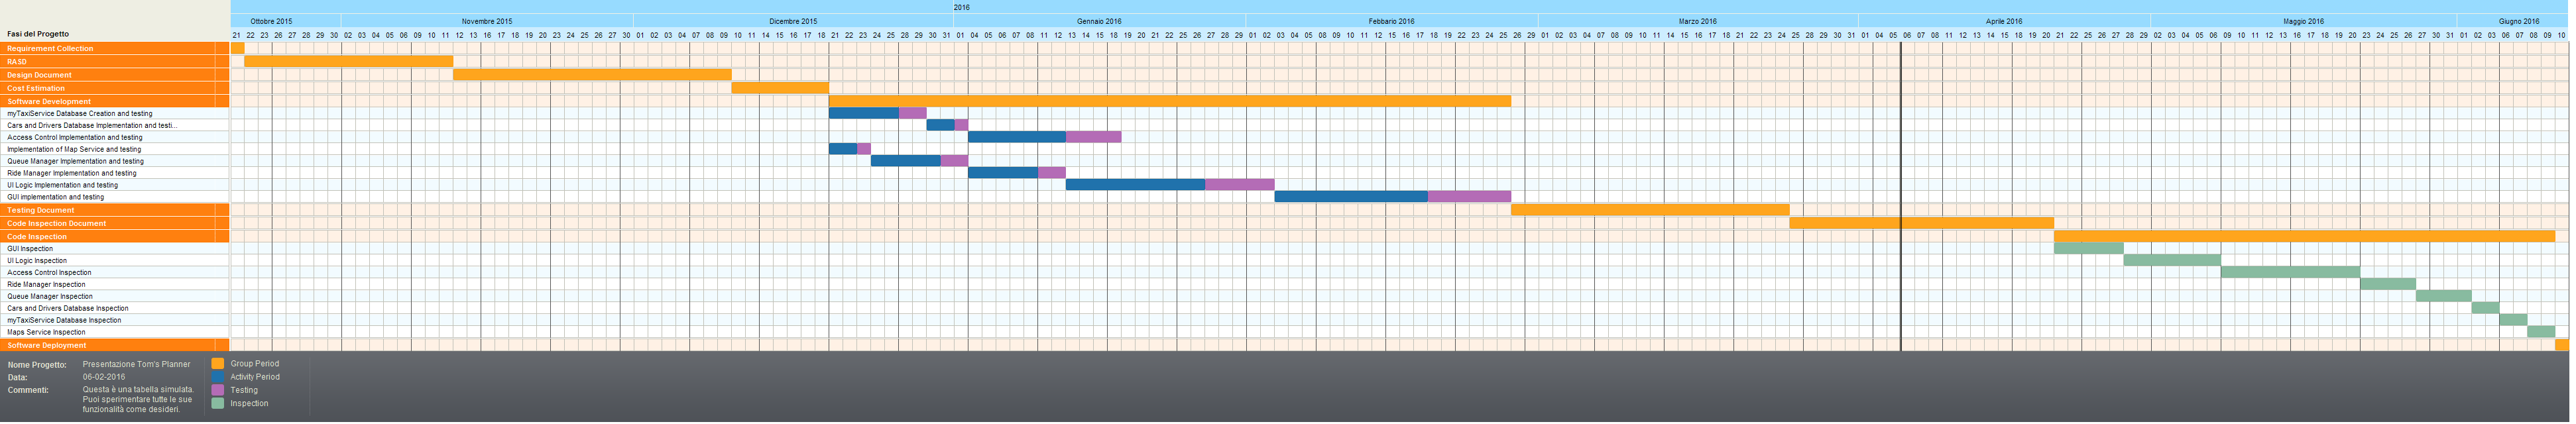
\includegraphics[scale=0.25]{DiagramSources/Ganttingsoftware2.png}
\label{Figure 1: }\caption{Gantt diagram of the project}
\end{figure}
\end{landscape}
In this section is presented the Gantt diagram of our project.\\
On 21\textsuperscript{st} October it has been set the meeting with the company that required us to project myTaxiService application. During that day, we talked about features and goals of the software to develop. We estimated the collection of this information requires only one day to be completed. \\
From the 22\textsuperscript{nd} of October to the 11\textsuperscript{th} of November we worked on RASD: using information gather during the meeting, we prepared the document to present it before the deadline. \\
Following Gantt diagram, it is possible to see that we continued our project writing the DD and like the previous document, we guaranteed the applicants to complete it in more or less a month. \\
After these two documents, we thought it was the time to write the Project Plan document, keeping one month the time necessary to conclude and to present it. \\
Software development is the next task, we estimate this phase will last approximately two months taking into consideration code writing part and the testing one. \\
Composition of Testing document is the next step and it will last four weeks. It will contains all mistakes present in developed code. \\
We continue with Code Inspection document that will show how various components have to test each other. Two months are necessary to complete inspection phase. \\
At the end, we will deploy the software to the company on 10\textsuperscript{th} June. \\
The overall time requested to complete the project is eight months as we estimated. \\
As you can see from Gantt diagram, weekends are not considered working day (due to working laws).\\      
	\break
\section{Resources and task allocation}
	\newpage
\section{Project risks}
	\break
\begin{appendices}
\section{Tools}
\section{Hours of Work}
\end{appendices}
\end{document}